%\documentclass[review]{elsarticle}
\documentclass[]{elsarticle}
\usepackage{underscore}
\usepackage{tikz}
\usepackage{tikz-uml}
\usetikzlibrary{positioning}
\usetikzlibrary{calc}
\usetikzlibrary{shapes.misc}
\usetikzlibrary{through,arrows} % for circle of nodes ...

\newif\ifsummary
\summarytrue % or \draftfalse


\usepackage{local-tikz-style}

\usepackage{lineno,hyperref}
\modulolinenumbers[5]

\newcommand{\cd}[1]{ {\it #1} }%

\journal{Journal of \LaTeX\ Templates}

%%%%%%%%%%%%%%%%%%%%%%%
%% Elsevier bibliography styles
%%%%%%%%%%%%%%%%%%%%%%%
%% To change the style, put a % in front of the second line of the current style and
%% remove the % from the second line of the style you would like to use.
%%%%%%%%%%%%%%%%%%%%%%%

%% Numbered
%\bibliographystyle{model1-num-names}

%% Numbered without titles
%\bibliographystyle{model1a-num-names}

%% Harvard
%\bibliographystyle{model2-names.bst}\biboptions{authoryear}

%% Vancouver numbered
%\usepackage{numcompress}\bibliographystyle{model3-num-names}

%% Vancouver name/year
%\usepackage{numcompress}\bibliographystyle{model4-names}\biboptions{authoryear}

%% APA style
%\bibliographystyle{model5-names}\biboptions{authoryear}

%% AMA style
%\usepackage{numcompress}\bibliographystyle{model6-num-names}

%% `Elsevier LaTeX' style
\bibliographystyle{elsarticle-num}
%%%%%%%%%%%%%%%%%%%%%%%

\begin{document}

\begin{frontmatter}

\title{Using ISO standards to design a metadata registry for climate data}
%%\title{Elsevier \LaTeX\ template\tnoteref{mytitlenote}}
%%\tnotetext[mytitlenote]{Fully documented templates are available in the elsarticle package on \href{http://www.ctan.org/tex-archive/macros/latex/contrib/elsarticle}{CTAN}.}

%% Group authors per affiliation:
\author{Martin Juckes}
%%\author{Elsevier\fnref{myfootnote}}
\address{Rutherford Appleton Laboratory, Didcot, UK}
%%\fntext[myfootnote]{Since 1880.}

%% or include affiliations in footnotes:
%%\author[mymainaddress,mysecondaryaddress]{Elsevier Inc}
%%\ead[url]{www.elsevier.com}

%%\author[mysecondaryaddress]{Global Customer Service\corref{mycorrespondingauthor}}
%%\cortext[mycorrespondingauthor]{Corresponding author}
%%\ead{support@elsevier.com}

%%\address[mymainaddress]{1600 John F Kennedy Boulevard, Philadelphia}
%%\address[mysecondaryaddress]{360 Park Avenue South, New York}

\begin{abstract}
The climate modelling community collaborate globally to generate a coordinated portfolio of climate simulations which serve to advance scientific understanding and to support the Assessment process of IPCC. 
The interoperability of data products among the participating institutions is guaranteed by a detailed specification of the parameters to be archived and the associated metadata requirements.
This paper looks at the potential for increasing interoperability towards users outside this core community by expressing metadata requirements through the language of ISO standards on metadata registries. 
\end{abstract}

\begin{keyword}
Data registry\sep
Climate data management
\end{keyword}

\end{frontmatter}

\linenumbers




%% standards references not set well as stands ... can modify the titles or look for other styles in article-header.


%% beging document is embedded in article-header
%%\begin{document}

\section{Introduction}\label{sec:intro}

The CMIP6 Data Request provides detailed technical specifications of thousands of climate parameters which are being archived by climate modelling centres around the world as part of a global effort to update the set of reference climate simulations which guide global policy on climate change mitigation and adaptation. 

The DREQ is built on domain standards which have evolved with the CMIP project. In this paper we explore the feasibility and potential benefits associated with expressing
these specifications through ISO standards. 

The work cuts across a range of standards which are introduced in Section \ref{sec:iso} below, covering aspects of geospatial referencing, physical quantities, and the organisation and processes inherent in running a registry of metadata specifications. 

The expected benefits will be both in terms of inter-operability with other standards which deal with environmental information and also in terms of learning from and exploiting practises which are embedded in the ISO standards. 

We look at five principle areas of the activity.
Firstly, the description the overall orangisational structure and community interaction. This involves a broad and rapidly growing network,
with participants from hundreds of institutions and dozens of countries. The structure has evolved organically, always pressured by the rapid 
expansion of the global climate modelling activity and the societal pressures associated with growing awareness of the risks posed by anthropogenic climate change. One of the consequences of the broad and loosely [who contributes ...]


Secondly, the definition of data types, including specification
of multi-dimensional arrays which combine geospatial coordinates with additional domain specific dimensions.

Thirdly, the specifications of physical quantities and associated units. The DREQ includes thousands of different quantities, 
all of which are defined in and registered in the CF Convention. In order to increase interoperability with
other communities this paper develops a mapping from the terms in the data request to ISO standard quantities.

Fourthly, the overall design is framed using the Object Management Group's metamodeling standards. 

Finally, the standard for governance of IT can be used to describe the connection between decision centres and services.

\begin{figure}[h]
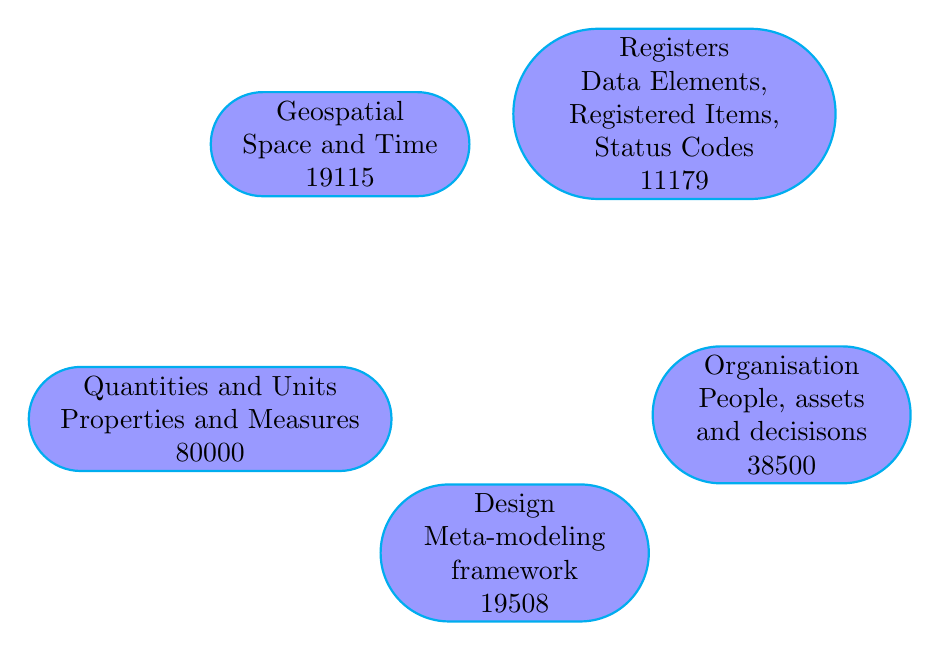
\begin{tikzpicture}[
  thick,
  every pin edge/.style={<-},
  >=latex,
  declare function/.list={
    outerR=2.0;,
    innerR=3.3;,
    angleofNode(\a)=\a/5*360-90;},
  std/.style={rounded rectangle, align=center, fill=blue!40, draw=cyan}
  ]

\node [circle through=(0:outerR)] (c) {};

\node[draw,std,anchor=angleofNode(2.5)] at (c.{angleofNode(0)}) {Design\\Meta-modeling\\framework\\19508};
\node[draw,std,anchor=angleofNode(3.5)] at (c.{angleofNode(1)}) {Organisation\\People, assets\\and decisisons\\38500};
\node[draw,std,anchor=angleofNode(4.5)] at (c.{angleofNode(2)}) {Registers\\Data Elements,\\Registered Items,\\Status Codes\\11179};
\node[draw,std,anchor=angleofNode(0.8)] at (c.{angleofNode(3)}) {Geospatial\\Space and Time\\19115};
\node[draw,std,anchor=angleofNode(1.5)] at (c.{angleofNode(4)}) {Quantities and Units\\Properties and Measures\\80000};

\end{tikzpicture}
\caption{The five core standards explored in this paper. The scope of these five standards overlaps in many areas, but
there do not appear to be any inconsistencies in the application discussed here.}
\label{fig:pentad}
\end{figure}

The ability to discuss the whole range of issues from governance to comprehensive technical details is a valuable 
strength of the ISO standards. This is of particular relevance in the context of a metadata registry which is
constructed through wide community engagement. Different categories of technical information require different
forms of approval and harmonisation. This paper aims to clarify the procedures, roles and responsibilities
through the ISO framework.


\subsection{Exploiting the International Standards Organisation [ISO]}\label{sec:iso}

[provisional literature notes]

\cite{sinaci2013} describes the ise of 11179 to facilitate exchange across clinical work and care domains.


The main pillars of the work will be: 

\paragraph{ISO 11179} \citep[Metadata Registry][]{Pon2009,iso80000-1} provides a framework for the organisational structure of a metadata registry and for
the technical specifications of the registers within that registry. Critically, this clarifies the decision processes and responsibilities surrounding 
the registration of new items. 

\cite{iso38500}

\cite{iso19508}

\begin{itemize}
\item QU-GE Quantities and Units (80000-1 {General})
\item QU-ST Quantities and Units (80000-3 {Space and Time})
\item QU-ME Quantities and Units (80000-4 {Mechanics})
\item QU-TH Quantities and Units (80000-5 {Thermodynamics})
\item QU-AC Quantities and Units (80000-7 {Light and Radiation})
\item QU-NP Quantities and Units (80000-9 {Physical Chemistry and Molecular Physics})
\item GI-DS  Geographic Information (19115-1 {Dataset})
\item GI-MD  Geographic Information (19115-1 {metadata})
\item MDR Metadata Registries (11179)
\end{itemize}

{\bf NB -- currently using old 80000-4: new version August 2019.}

MD_Metadata describes aspects of datatype, including information about accuracy of georeferencing which of importance in observational contexts.
Dimensions are present as unordered associates of the MD_Metadata class, with a sequence number. Key information is repeated. 


Here are two sample references: \cite{iso80000-1}.

\cite{iso19135-1} provides information on geospatial referencing.

\ifsummary
 %% [additional content omitted]
\else
\section{Overview of the metadata structures}

\subsection{Activities and Roles}\label{sec:roles}

\documentclass[tikz,border=10pt]{standalone}
\usepackage{tikz-uml}
\usetikzlibrary{positioning}
\usetikzlibrary{calc}

\tikzset{
  pck/.style = {
    minimum width = 3cm,
    node distance=2in,
    },
  note/.style = {
    width = 6cm,
    }
  }

\begin{document}

\begin{tikzpicture}

\begin{umlsystem}[x=4, fill=red!10]{The data request registry}
\umlusecase [name=AA] {Registry}
\umlusecase [below = 1cm of AA, name=A] {Register Collection}
\umlusecase [below = 1cm of A, name=B] {Register}
\umlusecase [below right = 0.5cm and 1cm of B, name=dec] {Item Specs}
\umlusecase [below left = 0.5cm and 1cm of B, name=ri] {Registered Item}
\umlusecase [x=2cm,y=-3cm, name=mon] {Monitor}
\end{umlsystem}

\umlactor[x=-2cm,y=0.5cm]{registrar}
\umlactor[x=-2cm,y=-1.5cm]{programme}
\umlactor[x=-2cm,y=-3.5cm]{pi}
\umlactor[x=-2cm,y=-5.5cm]{experts}
\umlactor[x=8cm,y=-3cm]{oversight}

%% would be nice to place stereotype above line ... probably need to change anchor .... occurs dozens of times in style file
%% should be straight mapping of code used for "stereo pos"
%% can use arg1, arg2, mult1, mult2 for additional info, but quickly becomes crowded
%%
\umlassoc[draw=black!50, very thick, arg1=operate,stereo=own]{registrar}{AA}
\umlassoc[arg1=govern,stereo=coordinate]{programme}{A}
\umlassoc[arg1=define,stereo=ipr]{experts}{ri}
\umlassoc{pi}{B}


\end{tikzpicture}

\end{document}



\subsection{Metadata Packages}\label{sec:packages}

\begin{figure}[p]
\begin{tikzpicture}


\begin{umlpackage}[fill=green!20]{Metadata}
\begin{umlpackage}[]{Parameters}
\umlsimpleclass[sc1,y=0]{units}
\umlsimpleclass[sc1,y=-0.8cm]{quantities}
\umlsimpleclass[sc1,y=-1.6cm]{constraints}
\umlsimpleclass[sc1,y=-2.4cm]{variables}
\end{umlpackage}

\begin{umlpackage}[]{Data Axes}
\umlsimpleclass[sc1,x=5cm,y=0]{axes}
\umlsimpleclass[sc1,x=5cm,y=-1cm]{coordinates}
\umlsimpleclass[sc1,x=5cm,y=-2cm]{configurations}
\end{umlpackage}

\begin{umlpackage}[]{Data Types}
\umlsimpleclass[sc1,x=5cm,y=-4.6cm]{\detokenize{data-type}}
\umlsimpleclass[sc1,x=5cm,y=-5.4cm]{spatial-grid}
\umlsimpleclass[sc1,x=5cm,y=-6.2cm]{temporal-grid}
\umlsimpleclass[sc1,x=5cm,y=-7cm]{\detokenize{cell-methods}}
\end{umlpackage}

\begin{umlpackage}[]{Request}
\umlsimpleclass[sc1,x=0cm,y=-4.6cm]{variable-group}
\umlsimpleclass[sc1,x=0cm,y=-5.4cm]{experiment-group}
\umlsimpleclass[sc1,x=0cm,y=-6.2cm]{objective}
\begin{umlpackage}[fill=black!10]{Choices}
\umlsimpleclass[sc1,x=0.4cm,y=-8.0cm]{options}
\end{umlpackage}
\end{umlpackage}

\begin{umlpackage}[]{Imports}
\umlsimpleclass[sc1,x=0cm,y=-10.2cm]{MIP}
\umlsimpleclass[sc1,x=0cm,y=-11cm]{standard-name}
\umlsimpleclass[sc1,x=5cm,y=-10.2cm]{experiment}
\end{umlpackage}


\end{umlpackage}

%%% Request .. linking
%%% Experiment ... [obsolete ... only need a class with links to experiments]
%%% Data types (structure).
%%% Data axes (structure).
\end{tikzpicture}
\caption{The metadata package is split into 5 sub-packages characterised by different harmonization and conformance requirements and mechanisms.}
\label{fig:packages}
\end{figure}

\subsection{The Metadata Region of MDR}\label{sec:mdrmdr}

MDR-3 [How to refer?] provides the framework for specifying the metadata requirements for "registered items". In this case the objective is to specify the requirements for datasets which will be archived and distributed through the ESGF distributed archive. The \cd{MDR:Data Entitity} class which provides the registry component of the specifcations of these datasets corresponds to the \cd{DREQ:CMORvar}, a record defining a physical variable sepcified as a mutli-dimensional field spanning time, space and potentially, other dimensions
such as wavelength, land cover type, ...

The \cd{DREQ:CMORvar} defines a range of properties such as the temporal sampling frequency and spatial processing requirements (e.g. masking and averaging), in addition to the structure of the field and the specification of the physical property.

In the new framework, these metadata elements are distributed among \cd{datatypes}, \cd{classifications}, \cd{descriptions}, \cd{value domain subsets} [[not sure if the last is needed]]

The information relevant to the \cd{datatype} is specified in terms of concepts from the CF Conventions which build on the NetCDF data model of arrays, dimensions and attributes.


\section{Quantities and Units of Measure}

The concept of "quantity" is discussed in 19115, 11179 and 80000 (where it is the main focus of the standard). In all cases, a "quantity" is physical property which can be expressed via a measure.

The 19115 and 80000 define a range of specific quantities, and 11179 defines a framework for defining additional quantities. There is some
duplication between 19115 and 80000. Where possible we will use terms defined in 19115.

In both 19115 and 80000, the quantities defined generally have a broader scope that the variables defined in DREQ. For instance, the ISO 80000 quantity "Thermodynamic Temperature" corresponds to 33 different DREQ variables, such as "Near-Surface Air Temperature", "Temperature at Snow-Ice Interface".

There are 7 quantities from 19115 which are used (implicitly) in DREQ: angle, scale, distance, speed, area, volume, weight.

From 80000 the following: acceleration, time (duration), pressure, surface density, mass density, kinematic velocity, mass flow rate,
heat flow rate, density of heat flow rate, Celsius temperature(*), thermodynamic temperature, attenuation rate, mass fraction,
volume fraction, amount-of-mass fraction, amount-of-substance concentration.

These come from parts 3 (Space and Time), 4 (Mechanics), 5 (Thermodynamics), 7 (Light and Radiation) and
9 (Physical chemistry and molecular physics) of the standard.

(*) "Celsius temperature" could, according to the guidance given in ISO 80000, be considered as the same quantity as thermodynamic temperature. They only differ by a fixed offset.

The parameters in DREQ which do not appear to fit any of the specific quantities defined in ISO 11179 or ISO 80000 will be defined covered by defining new quantities as registered items in a consistent style and granularity. For instance, energy flow, temperature flux, stress, pressure tendency. 

In this way, it is possible to express the portfolio of parameters in around 100 quantities. Labelling the parameters with appropriate ISO quantities is likely to increase interoperability with other archives supporting fields, such as engineering or medicine, which may be involved in climate mitigation, adaptation or emergency response.

\section{Data Types}

The aim here is to establish a pathway to formal description. Implementation will continue to be via the CF and NetCDF structures.

It would be possible to develop a complex data type representing the full range of information required in a dataset. This consists of the required data array, the coordinates used to represent the data, and ancillary variables. 

An alternative approach is to represent the data requested as a MDR_data_entity with associated MDR_sub_data_entity concepts, such that each individual element corresponds to a single array of data.

This latter approach conforms to GI-MD. 

The top level data entity is a record specifying the dimensions of all the required arrays, some of which may be user specified.
e.g.
\begin{verbatim}
parametric data type: 
      type dimensions (lat: integer, lon: integer, time: integer ) = 
             record ( lat, lon, time, bnd=2);
\end{verbatim}
or perhaps, the data array ...
\begin{verbatim}
parametric data type:
      type data (lat: integer, lon: integer, time: integer ) =
             array ( 1..lat, 1..lon, 1..time) of real(8,64);
\end{verbatim}


The data field itself will then be held in a sub data entity,
\begin{verbatim}
parametric data type: type data = array (1...PA_time,1...PA_lon,1...PA_lat) of real(8,64);
\end{verbatim}

Additional sub-data entity elements will contain data for the dimensions and the ancillary variables.
This approach allows a fairly direct mapping of DREQ records into data entity concepts, but draws the \cd{dimensions}/\cd{data} data type into the 
top level data entity.

At this point the details of the mapping are not as important as the demonstration that the mapping is feasible. 


Base data types are perhaps more easily specified in CDL, but need to define a templating syntax. - use PEP 3101.
The values to be replaced are placed in braces, e.g. "{n:d}" should be replaced by the value of "n" using the formatting designated by "d" (a "decimal integer").



%% perhaps a table of class vs. attribute list {as itemize env}, showing data type and attributes. e.g. long_name : c"Near Surface Air-Temperature", where the 'C"..."' denotes a data entity with value given by the string

This extends \cd{MD_Dimension}

\begin{verbatim}
bounded latitude (n:integer,data:sequence) {
dimensions:
  integer lat = {n};
variables:
  double lat(lat);
     lat.standard name = "latitude";
     lat.units = "degree north";
     lat.long name = "latitude" ;
     lat.bounds = "lat bnds";
     lat.axes = "Y";
data:
  lat = {data};
}
\end{verbatim}
Note that in order to apply the POP 3101 templating rules \verb+sequence+ would need to be expressed as a string.

The "data" needs to be expressed as a string .... not really what we want to say.

This can be expressed in the language of 11404:

\begin{verbatim}
parametric data type: type bounded latitude(values: sequence of (real(256,64) ) = \
      record (values,name: "lat", \
             long name: "latitude", \
             lat.bounds,..) ;
\end{verbatim}


The \cd{NetCDF:double} datatype corresponds to ISO 11404 \cd{real(2,64)}, i.e. 64-bit floating point. The remaining parameters are key-value pairs which define the physical
interpretation of the datatype through the CF Convention.

With this approach, however, the attributes \cd{lat.units} etc become external to the administrative structure of the registry, only the bundled entity 
is explicitly represented.

Express Datatype as a subclass of {\cd MDR:Concept} and define records to accomodate ....

The required data type elements will be (1) simple dimension, bounded dimension (inc. coordinate), fixed simple dimension, (4) fixed bounded dimension.

There are 35 land surface types used to express masking requirements of data. Desirable to move these to a \cd{mask} record, and express the CMOR grid table via a method of the registry. 

Similarly, there are a significant number of ancillary variables ("a", "b", etc) which should be expressed in the data type. Also "orog", which is a 2-d field.

.e.g \cd{hybrid height half} requires \cd{a, b, a bnds, b bnds, orog}.

The bounds variables have dimensions (n,2), and the orog variable is the shape of the spatial grid.

We can, however, express the fact that "level" must be one of "hybrid half height, alternate hybrid sigma, ...".


\begin{verbatim}
parametric data type: type values_type(n: integer) = array (1...n) of real(8,64);

parametric data type: type regular_longitude(m: integer) = record (values(n),name,long_name,bounds,..) ;
parametric data type: type regular_lat_lon(n: integer, m: integer) = record (values(n,m),name,dimensions(regular_latitude(n),regular_longitude(m));
type name = string-literal selecting ("latitude");
\end{verbatim}


11179 allows data types to be specified via a reference to a document.

Here, we use the notation of 11404 to specify the datatypes, since the underlying standards do not provide a formal specification. [illustrative sample]

The \cd{DREQ:cell measures} atttribute contains a string which is to be transferred into the eventual data files,
but which also carries some inferred meaning which is derived from the CMIP6 data format specifications and naming rules. 

There are consistency rules.




\section{Conclusions}\label{sec:conc}

The mapping of the DREQ onto the ISO standards reveals areas where improvements can be made in terms of clarity of decisions making processes and a structured approach to definingthe attributes which characterise registered items.

There does not appear to be any inherent obstacle to full compliance, though it has not been the purpose of this paper to compile a full technical specification.

The \cd{structure} record in DREQ-1.0 contained a complex mix of metadata specifications.
Guided by MDR, this can be divided between specification of a data type and processing instructions.
The resulting split improves the clarity of the specifications.

\fi

\section{References}

\bibliography{ams}
\end{document}
